%This work is licensed under the Creative Commons Attribution-NonCommercial-NoDerivs 3.0 United States License. To view a copy of this license, visit http://creativecommons.org/licenses/by-nc-nd/3.0/us/ or send a letter to Creative Commons, 444 Castro Street, Suite 900, Mountain View, California, 94041, USA.

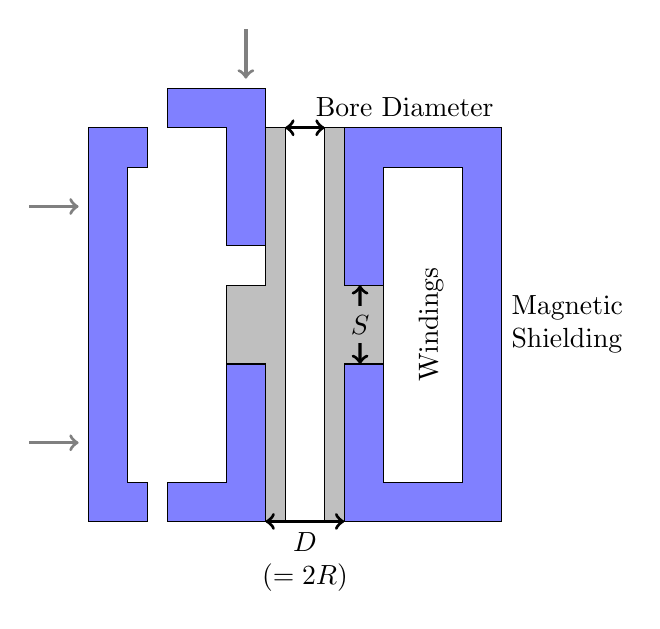
\begin{tikzpicture}
  \draw [fill=blue!50] 
    (-0.5,0.5)
    -- ++(0,2)
    -- ++(-1.25,0)
      node [pos=0.2] (assemble top) {}
    -- ++(0,-0.5)
    -- ++(0.75,0)
    -- ++(0,-1.5)
    -- ++(0.5,0)
    -- cycle
  ;

  \draw [very thick, <-, gray]
    (assemble top)
    -- ++(0,0.75)
  ;

  \draw [fill=blue!50]
    (-2,2)
    -- ++(-0.75,0)
    -- ++(0,-5)
      node [pos=0.2] (assemble left upper) {}
      node [pos=0.8] (assemble left lower) {}
    -- ++(0.75,0)
    -- ++(0,0.5)
    -- ++(-0.25,0)
    -- ++(0,4)
    -- ++(0.25,0)
    -- cycle
  ;

  \draw [very thick, <-, gray]
    (assemble left upper)
    -- ++(-0.75,0)
  ;
  \draw [very thick, <-, gray]
    (assemble left lower)
    -- ++(-0.75,0)
  ;

  \draw [fill=blue!50] 
    (-0.5,-1)
    -- ++(0,-2)
      coordinate [pos=1] (D left)
    -- ++(-1.25,0)
    -- ++(0,0.5)
    -- ++(0.75,0)
    -- ++(0,1.5)
    -- ++(0.5,0)
    -- cycle
  ;

  \draw [fill=blue!50] 
    (0.5,0)
    -- ++(0,2)
    -- ++(2,0)
    -- ++(0,-5)
      node [pos=0.5,right,align=left] {Magnetic\\Shielding}
    -- ++(-2,0)
    -- ++(0,2)
      coordinate [pos=0] (D right)
    -- ++(0.5,0)
    -- ++(0,-1.5)
    -- ++(1,0)
    -- ++(0,4)
    -- ++(-1,0)
    -- ++(0,-1.5)
    -- ++(-0.5,0)
    -- cycle
  ;

  \draw [fill=gray!50]
    (-0.5,2)
    -- ++(-0,-2)
    -- ++(-0.5,0)
    -- ++(0,-1)
    -- ++(0.5,0)
    -- ++(0,-2)
    -- ++(0.25,0)
    -- ++(0,5)
      coordinate [pos=1] (B left)
    -- ++(-0.25,0)
    -- cycle
  ;

  \draw [fill=gray!50]
    (0.5,2)
    -- ++(-0,-2)
    -- ++(0.5,0)
      coordinate [pos=0.4] (S top)
    -- ++(0,-1)
    -- ++(-0.5,0)
      coordinate [pos=0.6] (S bottom)
    -- ++(0,-2)
    -- ++(-0.25,0)
    -- ++(0,5)
      coordinate [pos=1] (B right)
    -- ++(0.25,0)
    -- cycle
  ;

  \draw [very thick,<->] 
    (S top) 
    -- (S bottom)
      node [pos=0.5,fill=gray!50] {$S$}
  ;
  \draw [very thick,<->] 
    (D left) 
    -- (D right)
      node [below,pos=0.5,align=center] {$D$\\$(=2R)$}
  ;
  \draw [very thick,<->] 
    (B left) 
    -- (B right)
      node [above right,pos=0.5,align=center] {Bore Diameter}
  ;
  \node [rotate=90] at (1.6,-0.5) {Windings};
\end{tikzpicture}
